% !TeX spellcheck = en_US
\documentclass[10pt,a4paper,notitlepage]{article}
\usepackage[utf8]{inputenc}
\usepackage{amsmath}
\usepackage{amsfonts}
\usepackage{amssymb}
\usepackage{graphicx}
%\usepackage[draft]{graphicx}
\usepackage{listings}
\usepackage{wasysym}
\usepackage[hidelinks]{hyperref}

\DeclareMathOperator*{\argmin}{arg\,min}

%opening
\title{Fast spectrum extraction \\
	{\small from DSLR and FITS images}}
\author{Christian Brock \footnote{Dresden Gönnsdorf Observatory}}
\date{ASPECT 2021 -- Lübeck}

\begin{document}

\setlength{\parindent}{0pt} 
\setlength{\parskip}{4pt} 

\maketitle

\tableofcontents

\begin{abstract}
	This paper presents a quick-and-dirty image processing pipeline that finds, de-rotates and visualizes the observed spectra.
	Finding, i.e. segmentation of the spectrum is accomplished with background removal using sigma clipping \cite{SigmaClipping}. The de-rotation angle is calculated from image moments \cite{ImageMoments}.
	The slit function as well as the spectrum are calculated from row averages and column-maxima of the de-rotated clipped image.
\end{abstract}

\section{Introduction}
	Exposure times are important, as under exposure reduces the SNR and over exposure invalidates the data.
	Finding correct initial exposure times or changing them due to variations in seeing conditions can be cumbersome.
	Often, especially for DSLR users this can be a manual process involving the use of image visualization software, e.g. Fitswork after the SD-card has been moved from the DSLR to a nearby computers. In our observatory the computer is located in a different room.
	
	In our observatory we fixed this issue:
	\begin{enumerate}
		\item We control our DSLR using gphoto2 \footnote{http://gphoto.org/}.
		\item In order to estimate the initial exposure time we calculate display image histograms for a range of time values (see figure \ref{fig:histograms}).
		\item For each science image we display the extracted spectrum image and the spectrum itself (see figure \ref{fig:spectra}).
	\end{enumerate}
	This article describes the third point above.

	\begin{figure*}[h]
	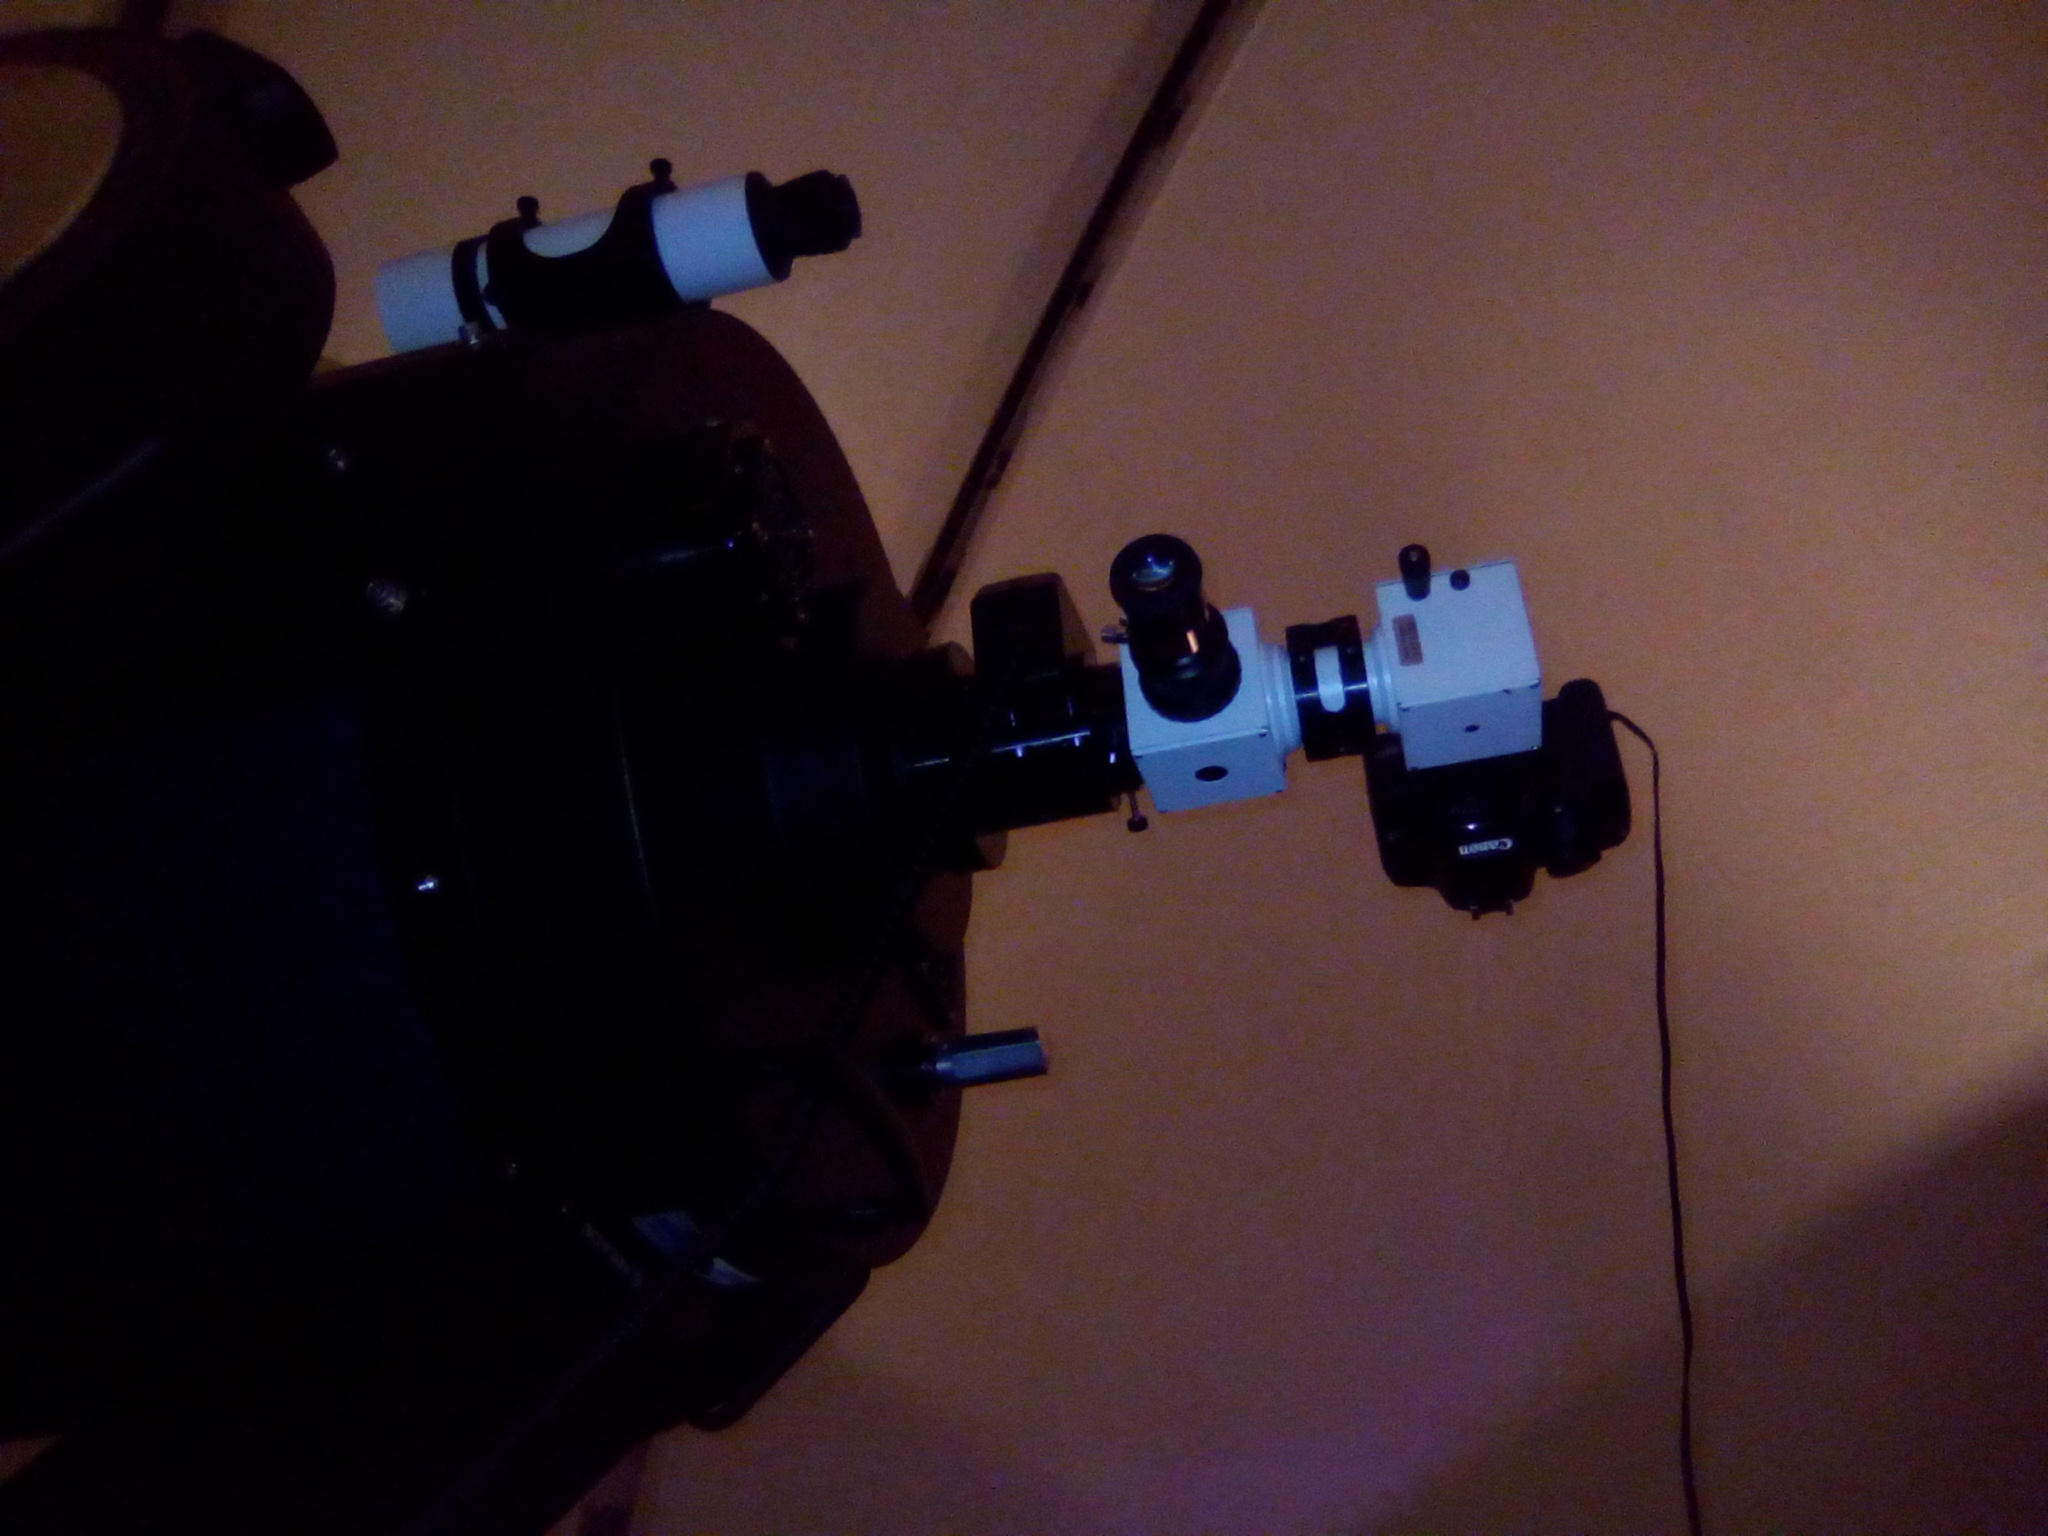
\includegraphics[width=0.49\columnwidth]{img/dados_nacht.jpg}
	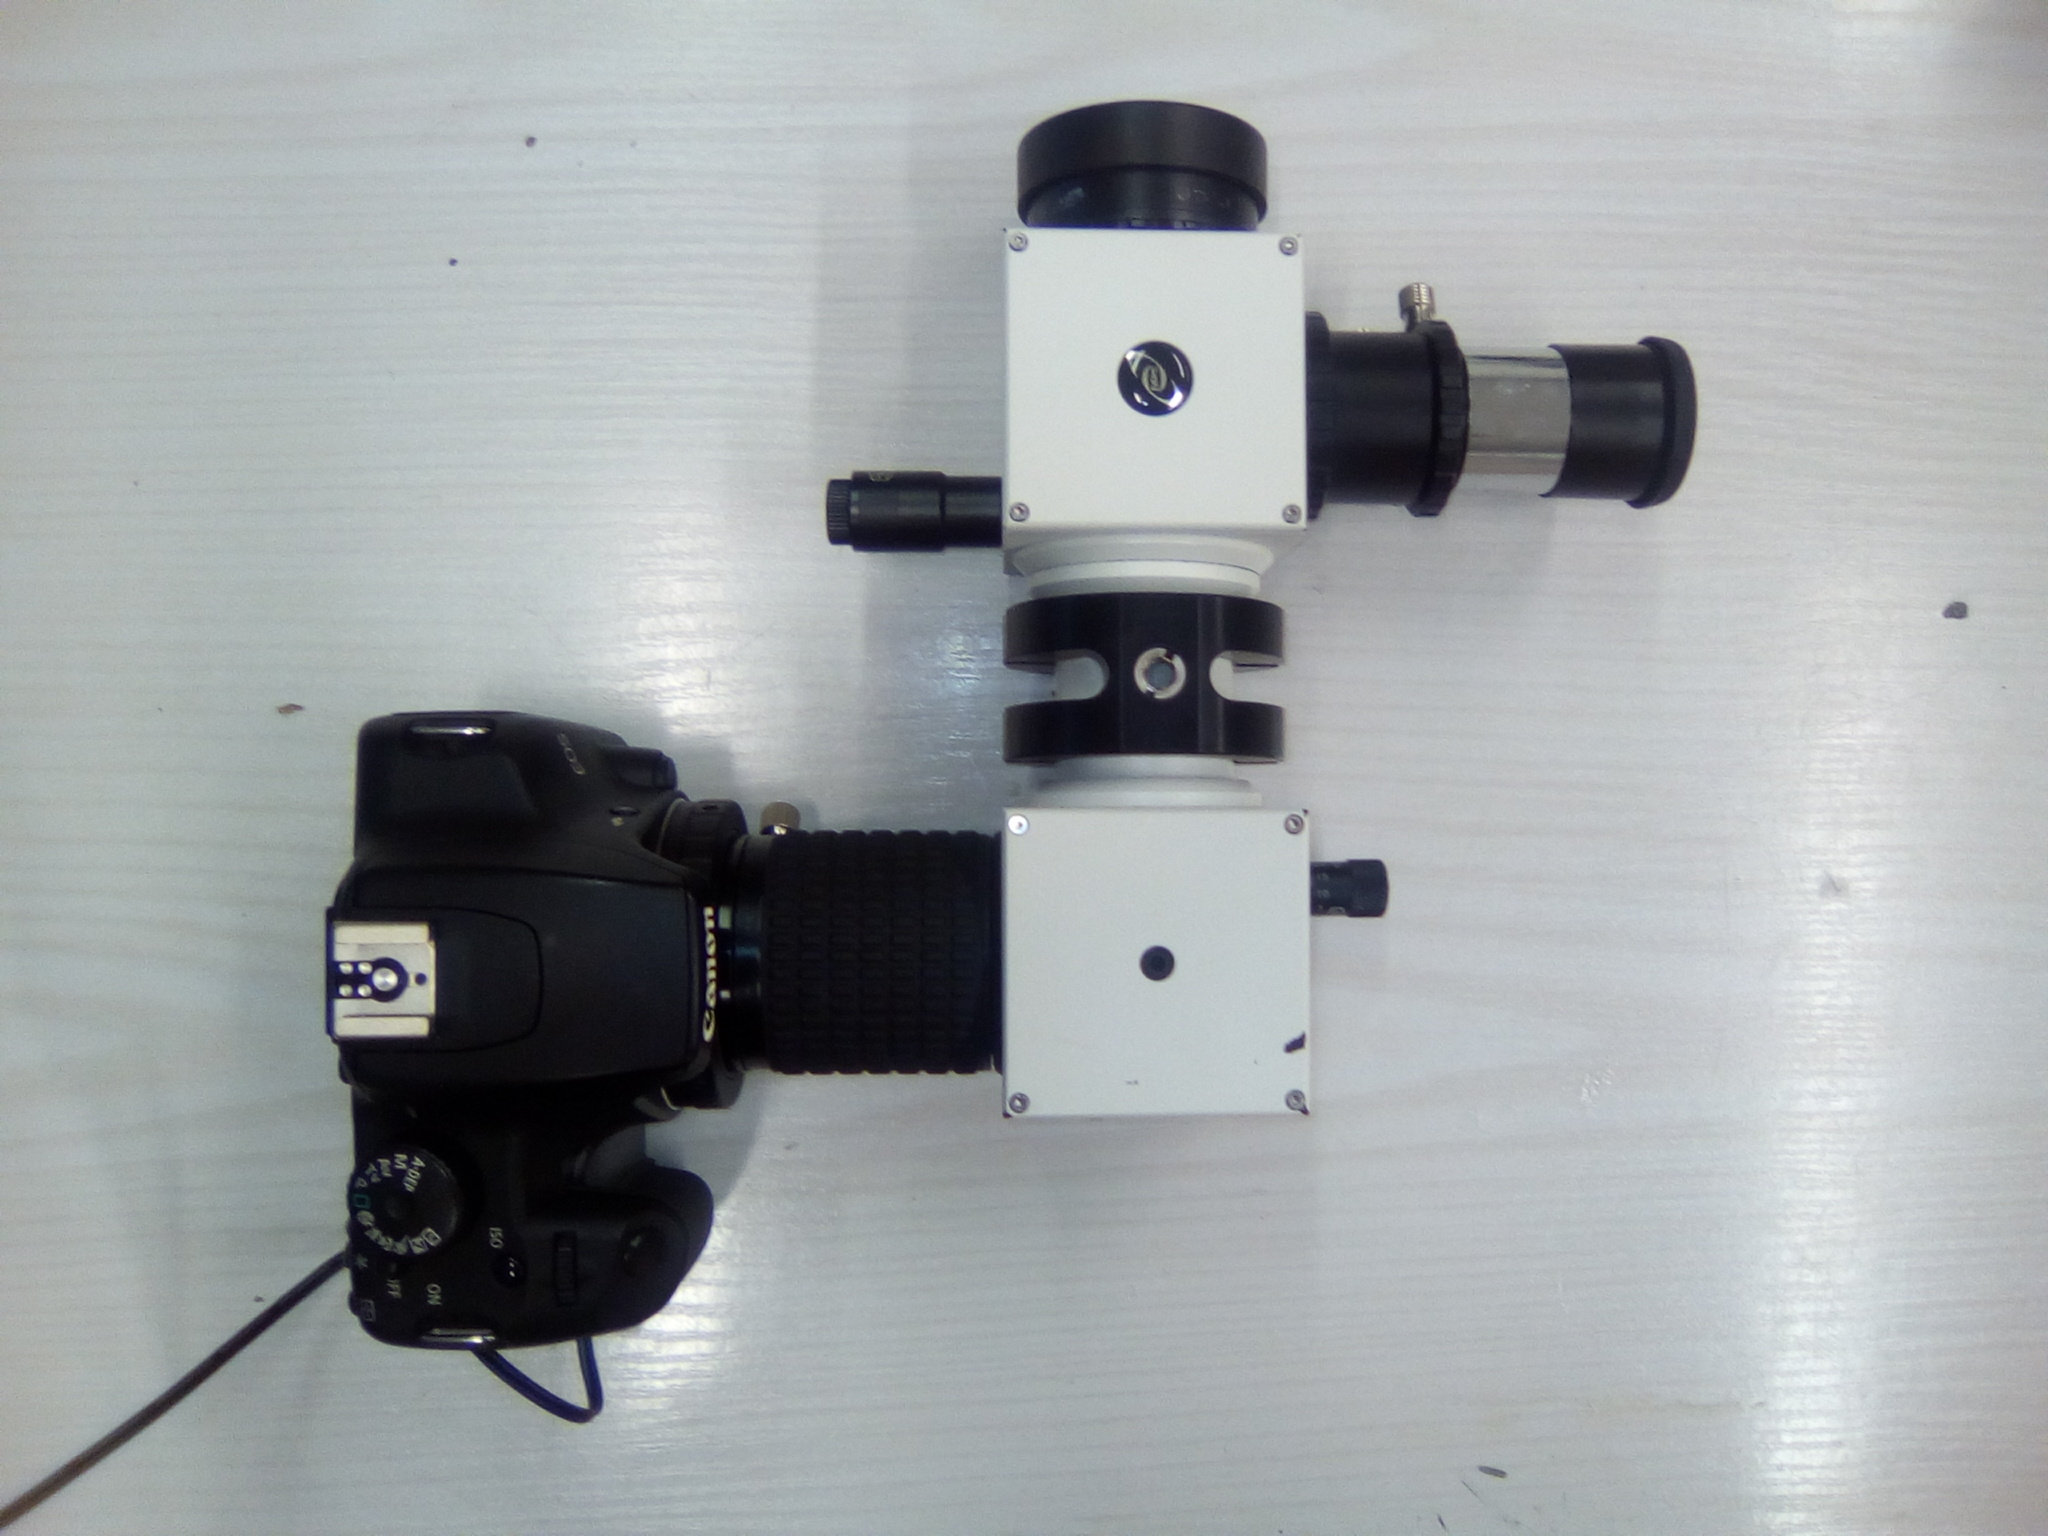
\includegraphics[width=0.49\columnwidth]{img/dados_tag.jpg}
	
	\caption[orig]%
		{Dados and Canon DSLR mounted on a Meade SC16 at the Dresden Gönnsdorf Observatory. Photos provided by Josefine Liebisch}
\end{figure*}
	

\section{Pipeline}
	
	To extract the spectrum from the image we need to 
	\begin{itemize}
		\item locate the spectrum in the image (see \ref{segmentation}) and
		\item detect whether the dispersion direction is tilted (see \ref{derotation}).
	\end{itemize}

	Slanting -- if the spectrum is not only rotated but projected in such a way, that it forms a parallelogram -- is out of scope of this paper.

	Once we have the image de-rotated and located we can extract the one dimensional spectrum as well as the slit function -- if needed (see \ref{extraction}).

	\subsection{Segmentation}
		\label{segmentation}
	
		Locating the spectrum in the image is a segmentation problem.
		In this pipeline we detect the image background with sigma clipping.
		Background mean ($\mu$) and standard deviation ($\sigma$) are computed by first computing $\mu$ and $\sigma$ for all image pixel $I_{xy}$ and then iteratively recompute $\mu$ and $\sigma$ for pixel with $I_{xy} \le \mu + N \sigma$.
		It can be easily shown that this iteration must converge at some $\mu_b$ and $\sigma_b$.
		Having $\mu_b$ and $\sigma_b$ we now discard all pixel $I_{xy} < \mu_b + M \sigma_b$.
		Remaining pixel belonging to the spectrum, are heavy noise or hot pixel.
		In the examples below $N$ and $M$ have been set to $3$ and $10$.

	\subsection{De-rotation}
		\label{derotation}
	
		If the camera is tilted in respect to the spectrograph it can be seen as a deviation of the dispersion direction of the spectrum from the row direction of the image.
		 
		With the result in \ref{segmentation} we can use image moments to calculate the tilt angle.
		The tilt angle is the angle between the largest eigen vector of covariance matrix
		$$\operatorname{cov}[I(x,y)] = \begin{bmatrix} \mu_{20} / \mu_{00} & \mu_{11} / \mu_{00} \\ \mu_{11} / \mu_{00} & \mu_{02} / \mu_{00} \end{bmatrix}$$
		 and the axis closest to that eigenvector where all $\mu_{xy}$ are central moments of the segmented spectrum.
		For further reading see \cite{ImageMoments}.
	
	\subsection{Extraction}
		\label{extraction}
	
		With the segmented and de-rotated image, we can again use image moments to find the center of gravity in slit direction $y$. It corresponds to the $y$-component of the centroid
		$$\bar{y} = M_{10} / M_{00}$$
		with $M_{xy}$ being the raw moments -- not to be confused with the central moments $\mu_{xy}$.
		The slit size can be derived from the second central moment in $y$-direction -- $\mu_{20}$.
		It means something like the variance of pixel coordinates in the slit direction.
		
		The extracted spectral images are displayed in figure \ref{fig:spectra}.
		
\section{Results}

	\begin{figure*}[h]
		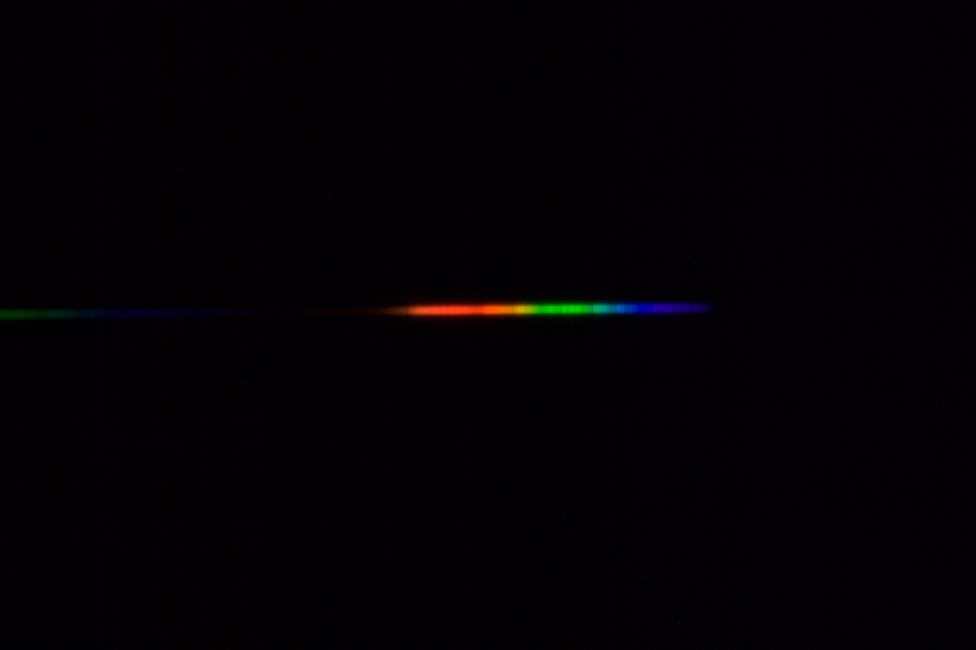
\includegraphics[width=0.49\columnwidth]{img/alpori.png}
		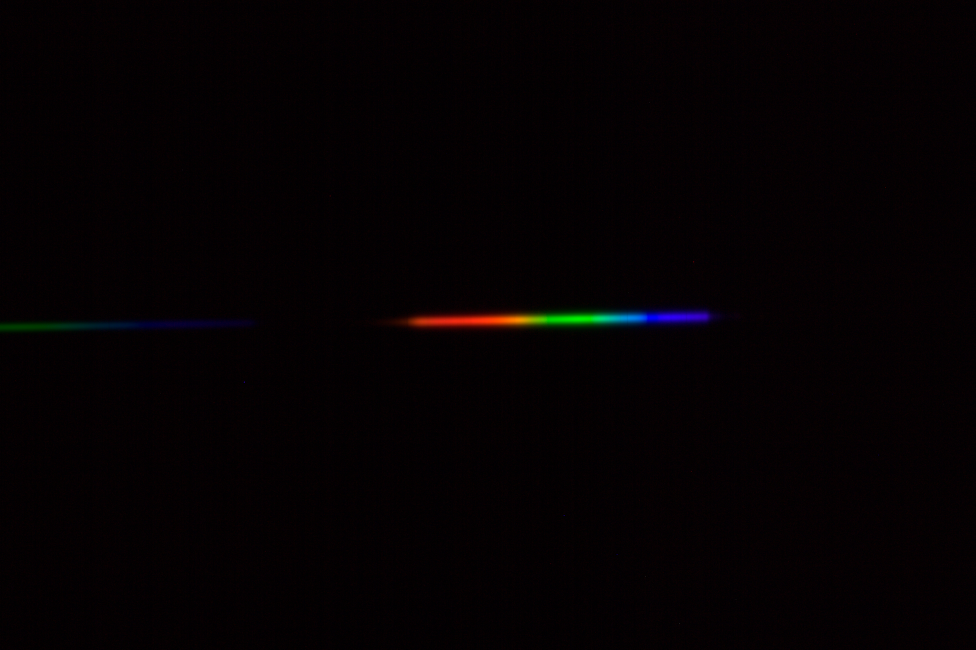
\includegraphics[width=0.49\columnwidth]{img/betori.png} \\
		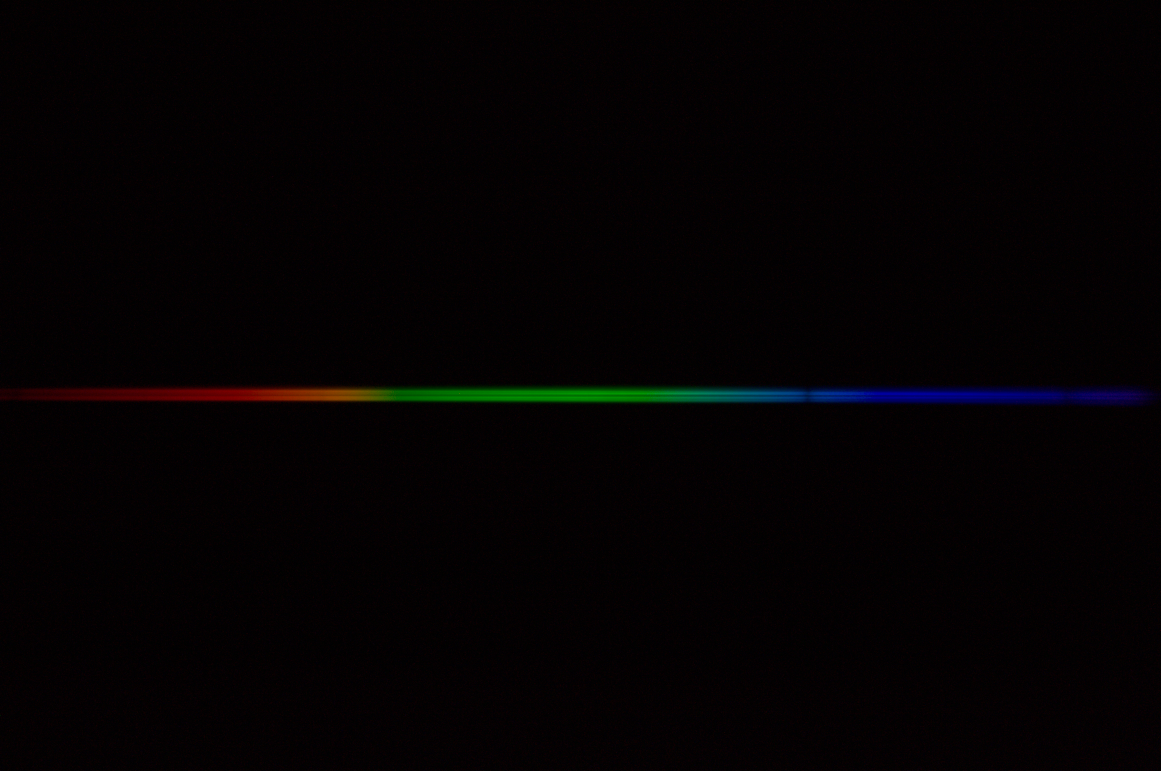
\includegraphics[width=0.49\columnwidth]{img/alpcma.png}
		
\includegraphics[width=0.49\columnwidth]{img/alpleo.png}
		
		\caption[orig]%
		{$\alpha$ Ori and $\beta$ Ori in the top row are captured with a Dados $200 l/mm$ grating and a Canon DSLR.
		$\alpha$ CMa on the bottom left was captured with a Dados $900 l/mm$ grating and a Nikon DSLR.
		The last FITS image came from Bernd Bitnar with a LHires and a Sigma 1603.}
		\label{fig:orig}
	\end{figure*}
	
	
	\begin{figure*}[h]
		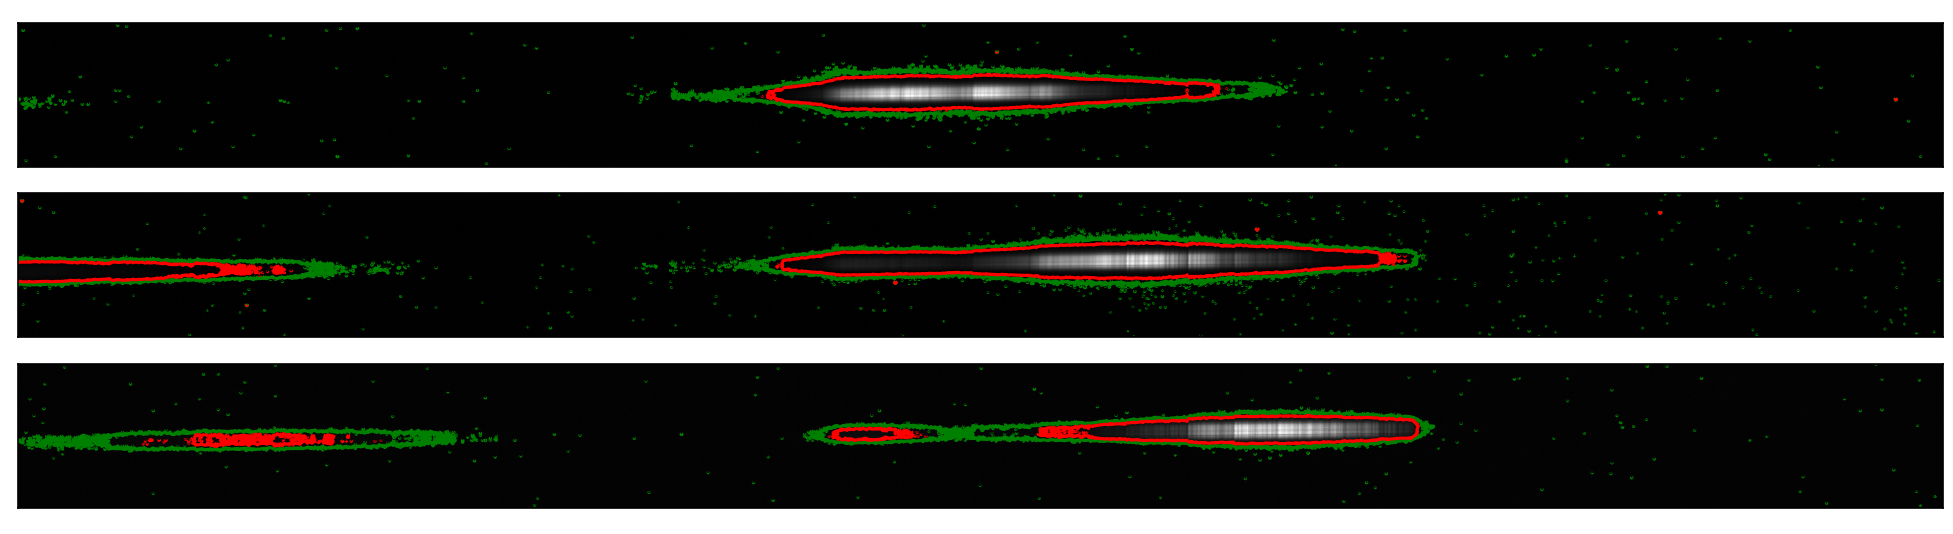
\includegraphics[width=\columnwidth]{img/alpori_segm.png} \\
		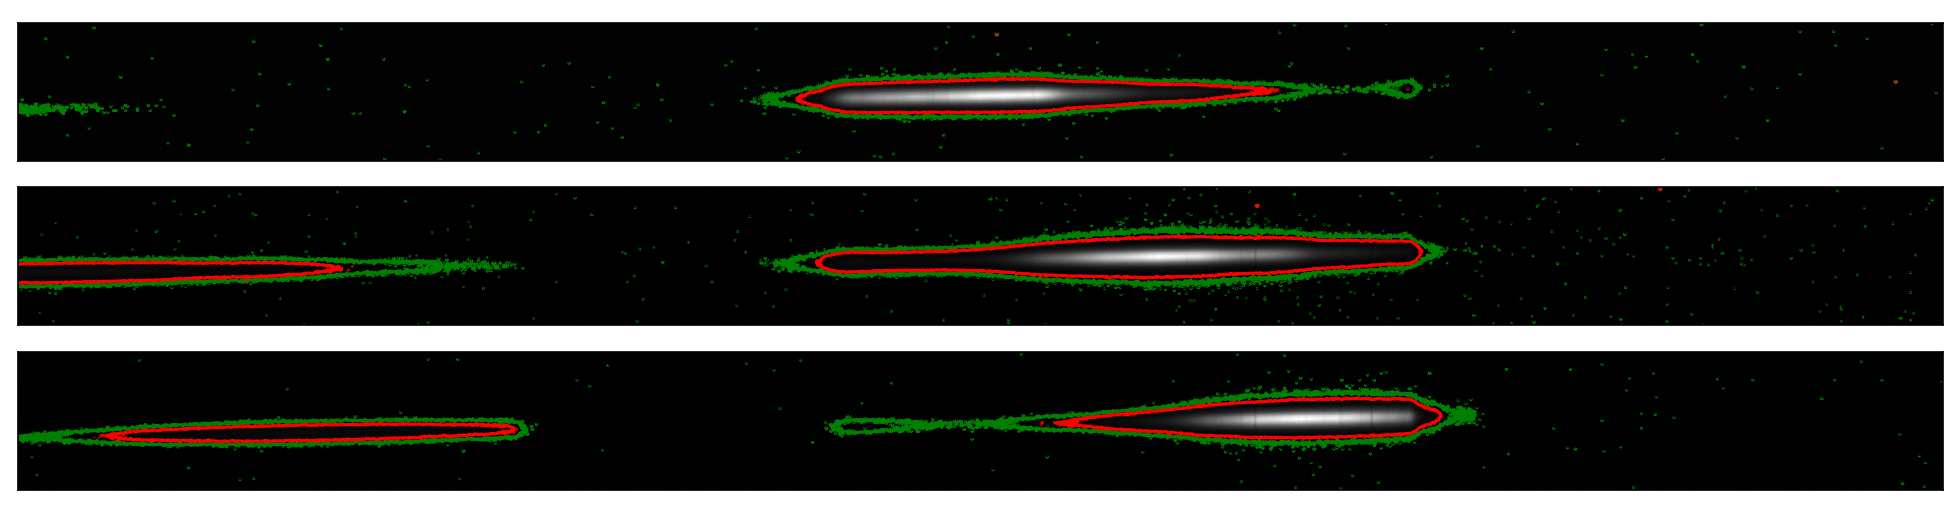
\includegraphics[width=\columnwidth]{img/betori_segm.png} \\
		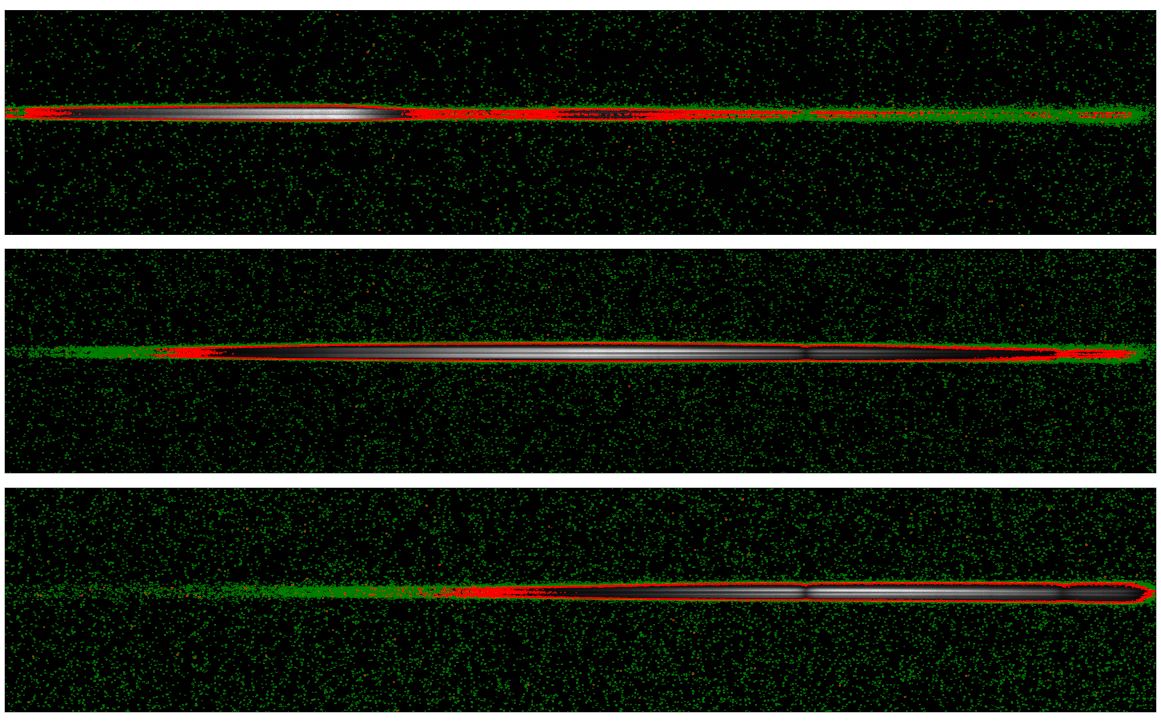
\includegraphics[width=\columnwidth]{img/alpcma_segm.png} \\
		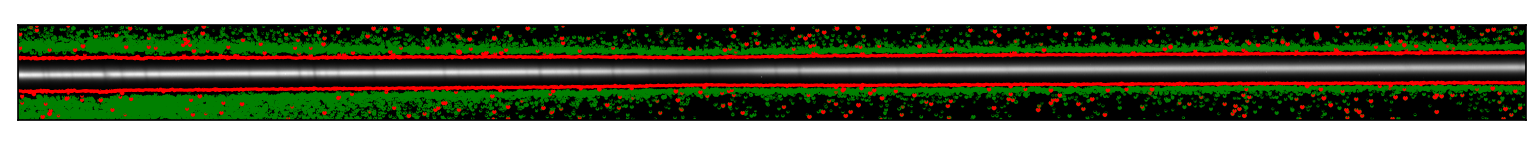
\includegraphics[width=\columnwidth]{img/alpleo_segm.png}		
		\caption[segmentation]%
		{Segmentation of image layers.
			The contours of $\mu_b + 3 \sigma$ are green and $\mu_b + 10 \sigma$ red.}
		\label{fig:segmentation}
	\end{figure*}

	\begin{figure*}[h]
		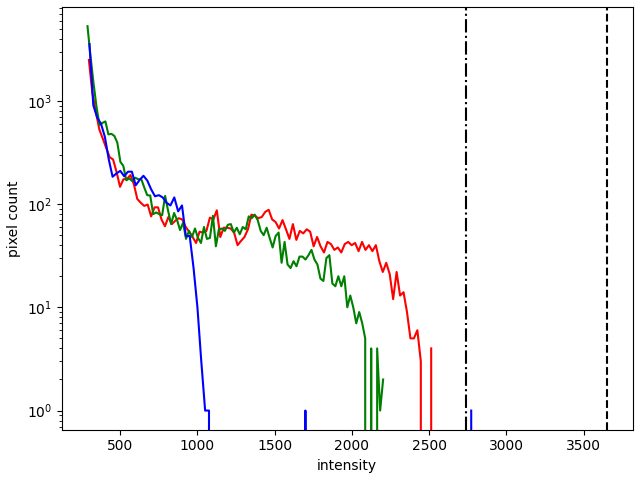
\includegraphics[width=0.49\columnwidth]{img/alpori_hist.png}
		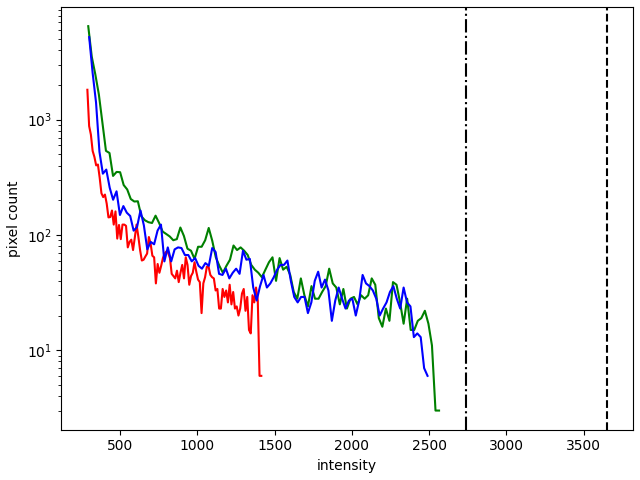
\includegraphics[width=0.49\columnwidth]{img/betori_hist.png} \\
		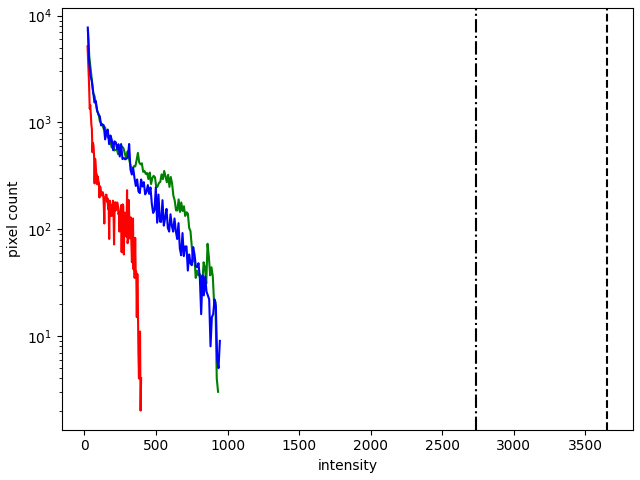
\includegraphics[width=0.49\columnwidth]{img/alpcma_hist.png}
		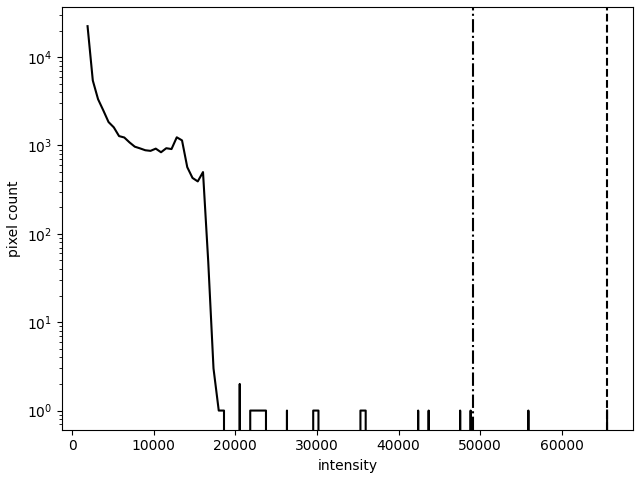
\includegraphics[width=0.49\columnwidth]{img/alpleo_hist.png}
		
		\caption[histograms]%
		{Pixel counts of the histograms are displayed on a logarithmic scale. Background pixel below $mu_b + 10\ \sigma_b$ are ignored. The vertical lines are placed at $75\%$ and full well depth.}
		\label{fig:histograms}
	\end{figure*}
	
	\begin{figure*}[h]
		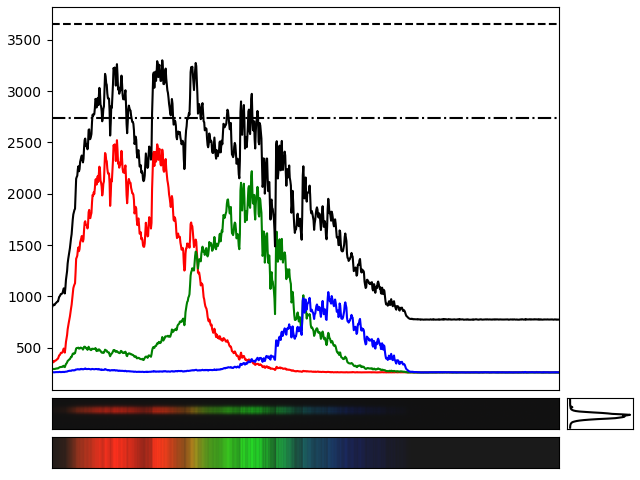
\includegraphics[width=0.49\columnwidth]{img/alpori_spec.png}
		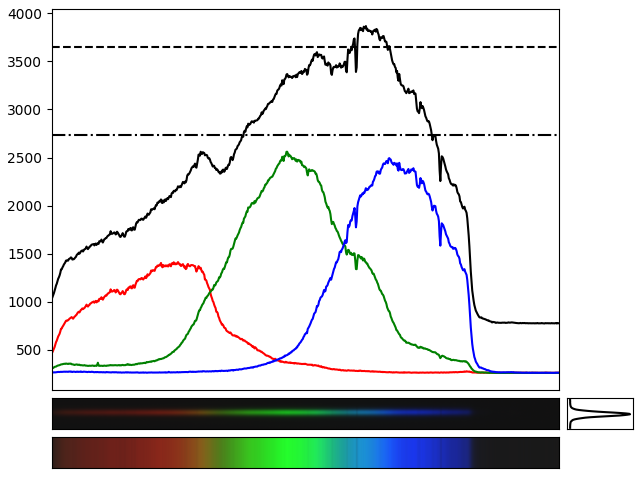
\includegraphics[width=0.49\columnwidth]{img/betori_spec.png} \\
		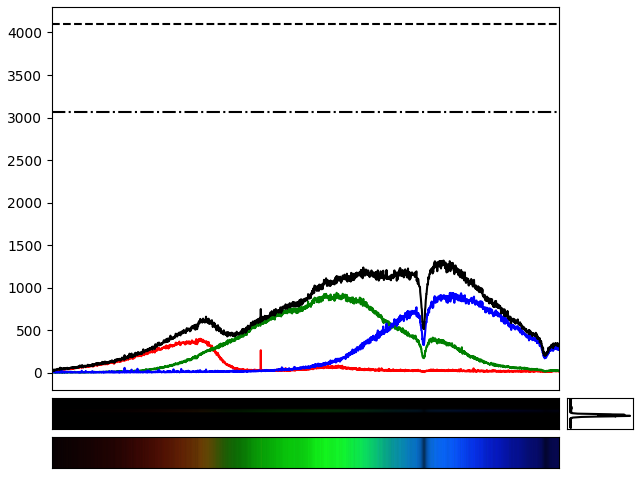
\includegraphics[width=0.49\columnwidth]{img/alpcma_spec.png}
		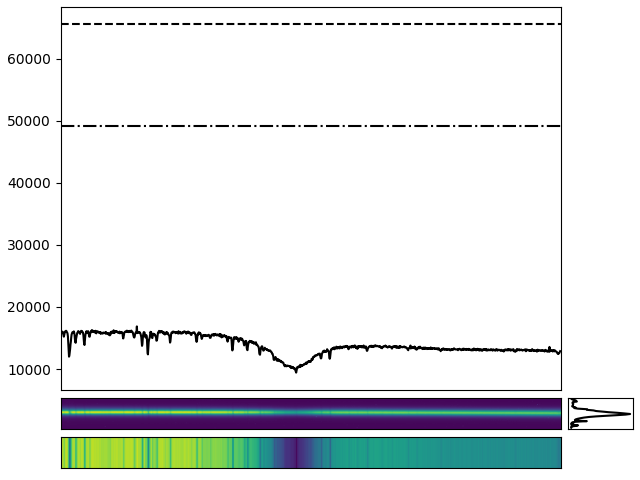
\includegraphics[width=0.49\columnwidth]{img/alpleo_spec.png}
		
		\caption[spectra]%
		{The extracted images, spectra and slit functions. For DSLR images, the sum of the three colors is displayed as black graph. The horizontal lines are placed at $75\%$ and full well depth.}
		\label{fig:spectra}
	\end{figure*}


\bibliographystyle{plain}
\bibliography{all}

\section*{About the author}
	During daytime Christian Brock programs algorithms to optimize cellular networks.
	At night he attends to visitors at the Dresden Gönnsdorf Observatory, mentors students, does some visual observations himself and cooperates in the Dresden spectroscopy group.

\end{document}
 